\documentclass[11pt]{article}
\input{/Users/markwang/.preamble}
\begin{document}


\section*{Diagnostics and Remedial Measures}


\subsection*{
    \href[page=124]{../apply_linear_model_kutner.pdf}{3.1} diagnostics for predictor variables}

\subsection*{
    \href[page=126]{../apply_linear_model_kutner.pdf}{3.2} 
    Properties of Residuals}


\begin{defn*}
    \textbf{Definition and Properties of residuals} \\
    residual $e_i$ is the difference between the observed value $y_i$ and fitted value $\hat{y}_i$
    \[
        e_i = y_i - \hat{y}_i
    \]
    so residual is a random variable and can be regarded as the \textbf{observed error}, in comparison to unknown true error $\epsilon_i$ in the regression model 
    \[
        \epsilon_i = y_i - \E(y_i)
    \]
    Note $\epsilon_i$ are assumed to be independent normal random variable with mean 0 and variance $\sigma^2$. If model is appropriate for the data at hand, then observed residual $e_i$ should reflect properties assumed for $\epsilon_i$. This underlies \textbf{residual analysis}, which is used to examine aptness of a statistical model
    \begin{enumerate}
        \item \textbf{mean} From taking partial of $RSS$ (when evaluating LS estimator)
        \[
            \overline{e} = \frac{\sum e_i}{n} = 0
        \]
        Note this does not imply $\E(\epsilon_i)=0$
        \item \textbf{Variance}
        \[
            s^2 = \frac{\sum(e_i - \overline{e})^2}{n-2}
            = \frac{\sum e_i^2}{n-2}
            = \frac{RSS}{n-2}
            = MSE
        \]
        if model is ok, MSE is unbiased estimator of $\sigma^2(e_i)$
        \item \textbf{nonindependence} residual $e_i$ are not independent random variables because they involve $\hat{y}_i$ which are based on the same fitted regression line. So residuals subject to 
        \[
            \sum e_i = 0 \quad \text{and} \quad \sum x_i e_i = 0
        \]
        If sample size is large, dependency effect of $e_i$ may be ignored
    \end{enumerate}
\end{defn*}

\begin{defn*}
    \textbf{semistudentized residuals} Want to standardize residual 
    \[
        e^*_i 
        = \frac{e_i - \overline{e}}{\sqrt{MSE}} 
        = \frac{e_i}{\sqrt{MSE}}
    \]
    if $\sqrt{MSE}$ is an estimate of $se(e_i)$, then $e_i^*$ is a \textbf{studentized residual}. But standard deviation of $e_i$ is complex, and $\sqrt{MSE}$ is only an approximation, so $e_i^*$ is \textbf{semistudentized residual}
\end{defn*}

\begin{defn*}
    \textbf{Possible departure from model with residuals}
    \begin{enumerate}
        \item regression fucntion is not linear 
        \item error term does not have constant variance (not homoscedastic)
        \item error term not independent 
        \item model fits all but one or a few outlier observations
        \item error term not normally distributed 
        \item one or several important predictor variables have been omitted from the model 
    \end{enumerate}
\end{defn*}


\subsection*{
    \href[page=127]{../apply_linear_model_kutner.pdf}{3.3} 
    Diagnostics for residuals}

\begin{defn*}
    \textbf{Nonlinearity of regression function} \\
    Deciding if a linear regression function is appropriate can be evaluated from a a \textbf{residual plot against $X$ or $\hat{Y}$}(preferred) or from a scatter plot. We look for if data points depart from zero in a systematic fashion \\ 
    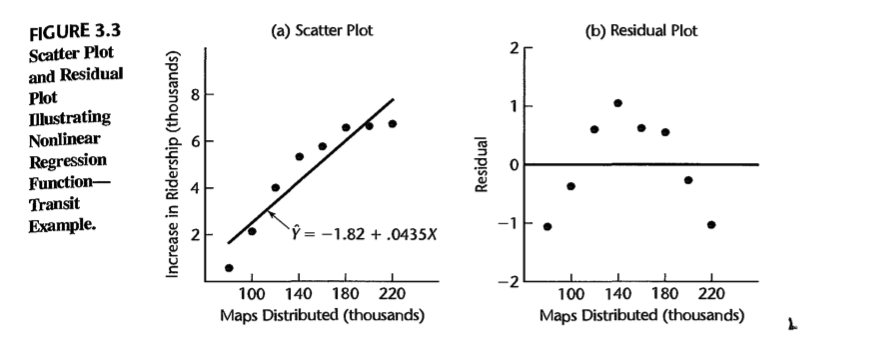
\includegraphics[width=\textwidth]{res_vs_predictor_plot.png}    
\end{defn*}

\begin{defn*}
    \textbf{Nonconstancy of error variance}\\
    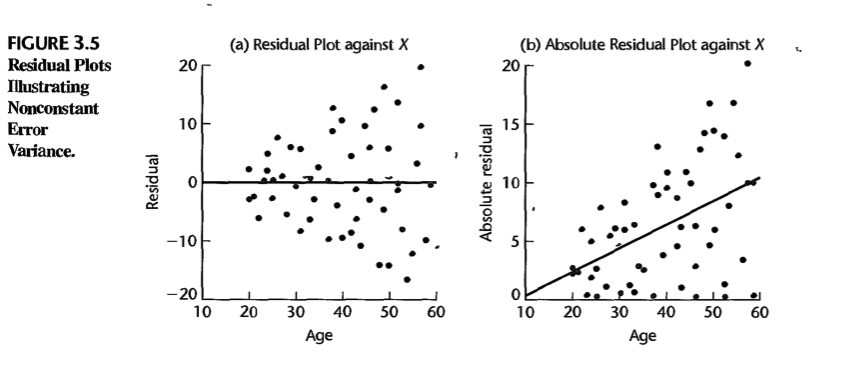
\includegraphics[width=\textwidth]{err_var_plot.png}    
\end{defn*}

\begin{defn*}
    \textbf{Presence of outliers}\\
    Can be examined from a \textbf{residual plot against $X$ or $\hat{Y}$} as well as 
    \begin{center}
        \textbf{plot of semistudentized residual}
    \end{center}
    The latter is useful in that its easy to identify residuals that lie many standard deviations from zero ($\geq$ 4 standard deviation may be considered outlier) \\ 
    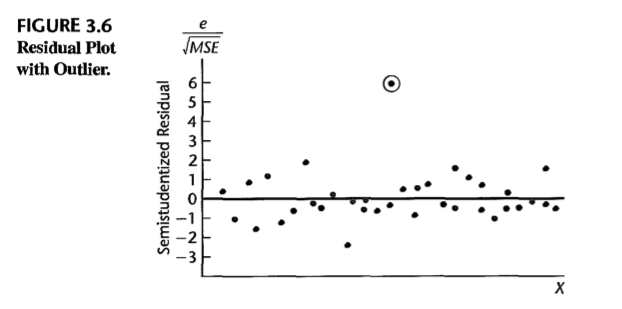
\includegraphics[width=\textwidth]{outlier_plot.png}    
    Outliers create difficulty for modeling. Since for least squared estimators, the fitted line may be pulled disproportionately toward an outlying observation, causing misleading fit if outlier is from a mistake or other cause
\end{defn*}

\begin{defn*}
    \textbf{Nonindependence of error terms} \\
    Whenever data obtained in a time sequence or some other type of sequence (geographical area), its good idea to use a \textbf{sequence plot of residuals} to see if there is correlation between error terms near each other in sequence. If error terms are independent, we would expect residuals in a sequence plot to fluctuate in a random pattern around base line 0\\
    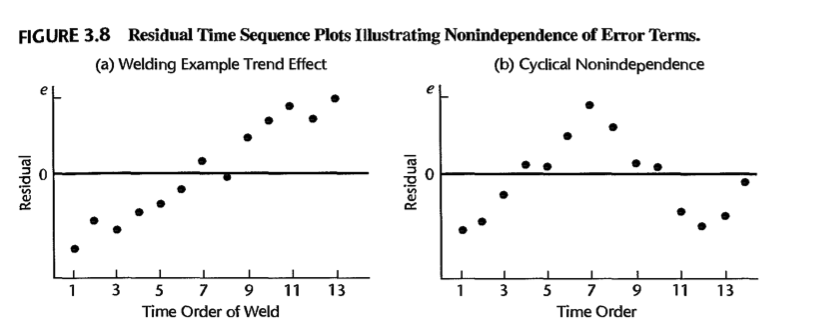
\includegraphics[width=\textwidth]{nonnidependence_plot.png}
\end{defn*}


\begin{defn*}
    \textbf{Nonnormality of error terms} \\
    Test with distribution plot, like \textbf{box plot} or \textbf{histogram}. Another possibility is to prepare a 
    \begin{center}
        \textbf{Normal probability plot}
    \end{center}
    where each residual is plotted against its expected value under normality. A plot that is linear suggest agreement with normality. \\
    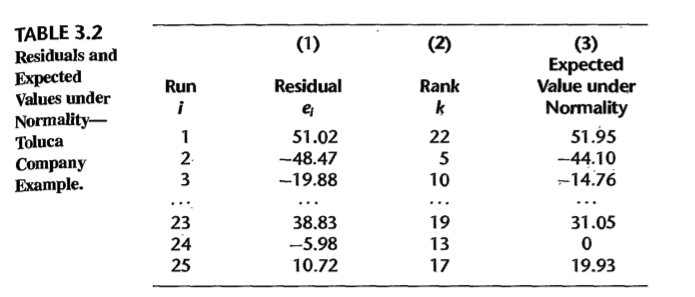
\includegraphics[width=\textwidth]{normal_prob_plot1.png} \\ 
    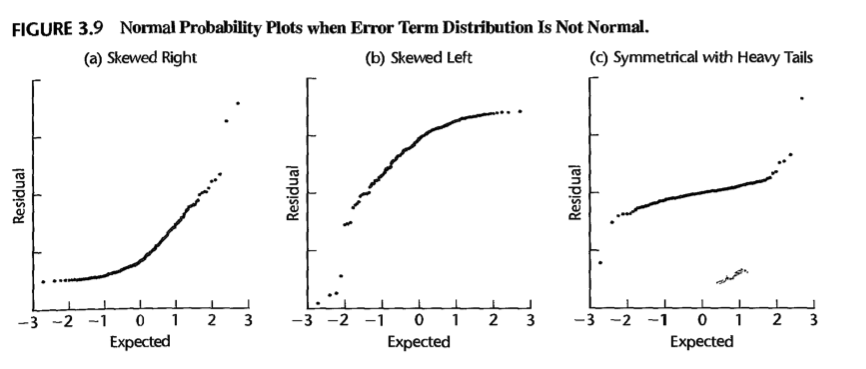
\includegraphics[width=\textwidth]{normal_prob_plot2.png} \\ 
    Heavy tail means that distribution has higher probabilities in the tails than a normal distribution. Note left skew distribution has a long tail to the left or graph (mean less than median)
\end{defn*}

\begin{defn*}
    \textbf{Omission of important predictor variables}\\
    Residuals should also be plotted agianst variables omitted from model that might have important effect on the model. Goal is to identify if there is other key variables in providing important additional predictive power to the model \\
    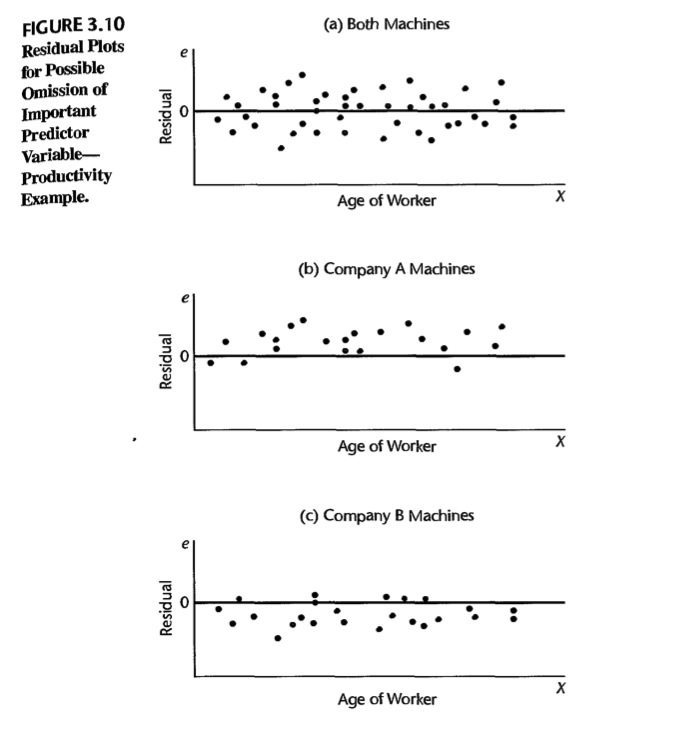
\includegraphics[width=\textwidth]{other_predictor_plot.png} \\ 
\end{defn*}



\subsection*{
    \href[page=138]{../apply_linear_model_kutner.pdf}{3.4} 
    Overview of Tests Involving residuals}



\subsection*{
    \href[page=161]{../apply_linear_model_kutner.pdf}{3.8} 
    Overview of Remedial Measures}




\subsection*{
    \href[page=153]{../apply_linear_model_kutner.pdf}{3.9} 
    Transformations}

\begin{defn*}
    \textbf{Transformation} \\
    Used to stablize nonconstant error variance, which usually helps with fixing nonnormality of error terms \\
    \begin{enumerate}
        \item 
        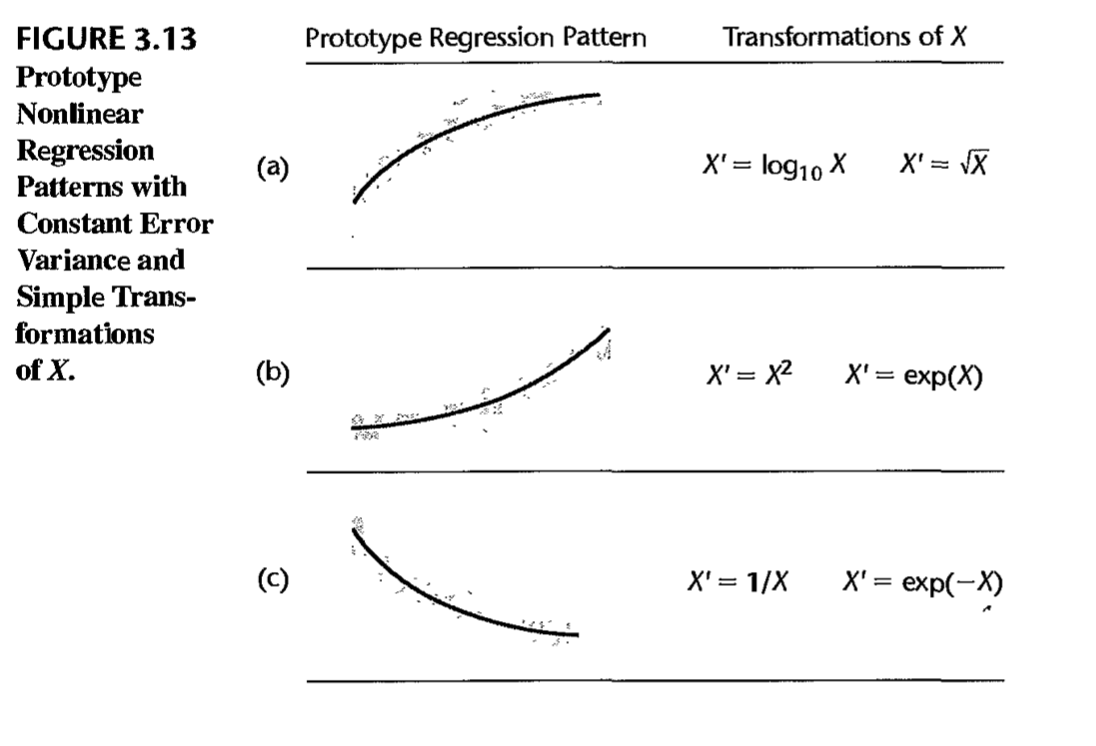
\includegraphics[width=\textwidth]{transformation_on_X.png}
        \textbf{Transformations for Nonlinear Relation Only} Used for linearizing a nonlinear regression relation when distribution of error term is reasonably close to a normal distribution and error terms have approximately constant variance. In this case, transformation on $X$ should be attempted (transformation on $Y$ may change shape of distribution of error term from normal and/or differing error term variances). Usually, we transform $X' = f(X)$ and refit the regression model, followed by checking if constant error variance, and error normality is maintained before and after the transformation
        \item 
        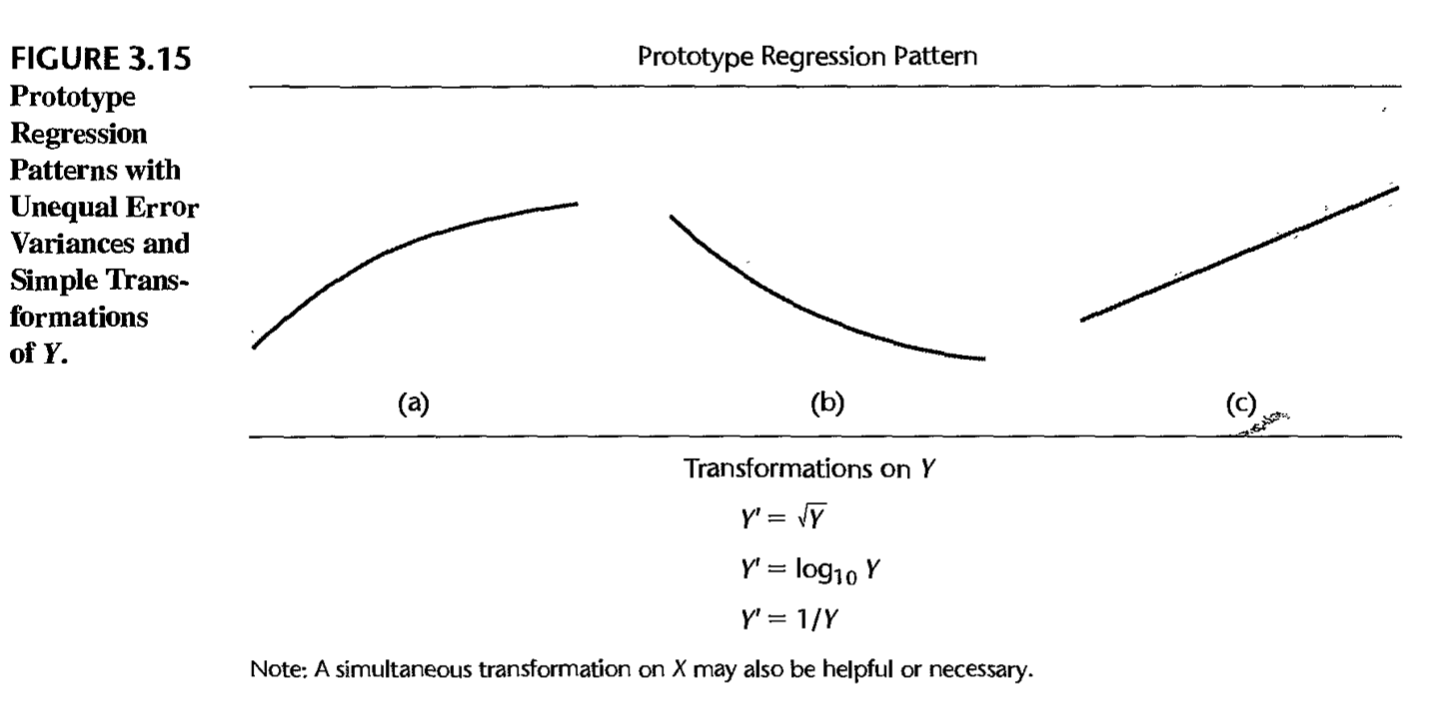
\includegraphics[width=\textwidth]{transformation_on_Y.png}
        \textbf{Transformation for Nonnormality and unequal error variances} Transformation on $Y$ affects shapes and spreads of distributions of $Y$, which in turn affects error variance/normality. Additionally, it may help linearize curvlinear regression regression. Frequently, there is \textbf{increasing skewness and increasing variability} of distribution of error terms as the mean response $\E(Y)$ increases
        \item \textbf{Box-Cox transformation} \\
        Infers te appropriate transformations of $Y$ for correcting skewness of distribution of error terms, unequal error variances, and nonlinearity of the regression. It identifies transformation from the family of power transformations on $Y$ 
        \[
            Y' = Y^{\lambda}
        \]
        such that we have regression model 
        \[
            Y^{\lambda} = \hat{\beta}_0 + \hat{\beta}_1 X_i + \epsilon_i
        \]
        with an additional parameter to estimate $\hat{\lambda}$ with MLE
    \end{enumerate}
\end{defn*}

\subsection*{
    \href[page=823]{../apply_linear_model_kutner.pdf}{18.5} 
    Transformation of Response Variables}


% \begin{defn*}
%     \textbf{Guides to finding a transformation} \\
%     Transformation on $Y$ that stablizes error variances 
%     \begin{enumerate}
%         \item \textbf{Variance Proportional to $\mu_i$} 
%     \end{enumerate}
% \end{defn*}



\subsection*{
    \href[page=434]{../apply_linear_model_kutner.pdf}{10.4} 
    Identifying Influential cases - DFFITS, Cooks distance, DFBETAS}

\begin{defn*}
    \textbf{Intro} After identifying cases that are outlying w.r.t. $Y$ and/or $X$ values, we have to ascertain if they are influential. A data point is considered \textbf{Influential} if its exclusion causes major changes in the fitted regression function
\end{defn*}

\begin{defn*}
    \textbf{Influence on single fitted value DFFITS}\\
    $DFFITS_i$ represents the difference between \textbf{fitted value} $\hat{y}_i$ for $i$th case when all $n$ cases are used in fitting regression function and the the \textbf{predicted values} $\hat{y}_{i(i)}$ for which the $i$th case obtained when the $i$th case is omitted in fiotting the regression function.
    \[
        (DFFITS)_i = \frac{\hat{y}_i - \hat{y}_{i(i)}}{se(\hat{y}_{i(i)})} \quad \text{where} \quad 
        se(\hat{y}_{i(i)}) = \sqrt{MSE_{(i)} h_{ii}}
    \]
    Note it uses $MSE_{(i)}$, the error mean square when $i$ the case is omitted in fitting the regression function for estiamting error variance $\sigma^2$. By standardization, $DFFITS_i$ represents number of estimated standard deviation of $\hat{y}_i$ that the fitted value $\hat{y}_i$ increases/decreases with the inclusion of $i$th case in fitting the regression model
\end{defn*}

\begin{defn*}
    \textbf{Influence on all fitted values - Cook's distance} \\
    Cook's distance considers influence of $i$th case on all $n$ fitted values, i.e. an aggregate influence measure, 
    \[
        D_i = \frac{\sum_j (\hat{y}_j - \hat{y}_{j(i)})^2}{pMSE}
    \]
    The larger the $\hat{e}_i$ and $h_{ii}$, the larger $D_i$. So $i$th case can be influential if 
    \begin{enumerate}
        \item have a large residual $\hat{e}_i$ and only a moderate leverage value $h_{ii}$ or 
        \item have a larger leverage value $h_{ii}$ but a moderately sized residual $\hat{e}_i$ 
        \item have both a large residual and a large leverage
    \end{enumerate}
\end{defn*}


\begin{defn*}
    \textbf{Influence on the regression coefficient DFBETAS} \\
    $DFBETAS_i$ is a measure of the influence of the $i$th case on each regression coefficient $\hat{\beta}_k$ ($k = 0, 1,\cdots$), specifically it is the difference between estimated regression coefficient $\hat{\beta}_k$ based on all $n$ cases and the regression coefficient obtained when $i$th case is omitted, denoted as $\hat{\beta}_{k(i)}$
    \[
        (DFBETAS)_{k(i)} = 
        \frac{\hat{\beta}_k - \hat{\beta}_{k(i)}}
            {se(\hat{\beta}_{k(i)})} 
        \quad 
        k = 0,1,\cdots, p-1 
        \quad \text{where} \quad 
        se(\hat{\beta}_{k(i)}) = \sqrt{MSE_{(i)}c_{kk}}
    \]
    where $c_{kk}$ is $k$th diagonal element of $(X'X)^{-1}$, so variance of $\hat{\beta}_k$ is given by 
    \[
        \sigma^2(\hat{\beta}_k) = \sigma^2 c_{kk}
    \]
    Note 
    \begin{enumerate}
        \item sign of DFBETAS indicates if inclusion of a case leads to an increase or a decrease in the estimated regression coefficient 
        \item absolute magnitude of DFBETAS indicate size of difference relative to estiamted standard deviation of regression coefficient. So large $DFBETAS_{k(i)}$ is indicative of large impact of $i$th case on $k$th regression coefficient 
        \item A case is \textbf{influential} if $|DFBETAS|$ exceeds 1 for small to medium datasets and $2 / \sqrt{n}$ for large datasets
    \end{enumerate}
\end{defn*}
    



\section*{
    \href[page=58]{../../modern_regression_with_r.pdf}{modern regression with r ch3} 
}
    
\subsection*{
    \href[page=58]{../../modern_regression_with_r.pdf}{3.1.2} Use residual plot to determine if proposed regression is a valid model }

\subsection*{
    \href[page=63]{../../modern_regression_with_r.pdf}{3.2}
    Regression diagnostics tools for checking validity of a model}
    
\begin{defn*}
    \textbf{Steps}
    \begin{enumerate}
        \item determine if proposed regression model is valid
        \begin{center}
            See if there is pattern in standardized residual plot
        \end{center}
        \item Identify \textbf{leverage points} 
        \begin{center}
            See if leverage $h_{ii}$ satisfies $h_{ii} > \frac{4}{n}$
        \end{center}
        \item Identify \textbf{outliers} 
        \begin{center}
            See if studentized residual $r_i$ satisfies $|r_i| > 2$
        \end{center}
        \item Identify \textbf{bad leverage points or influential points} 
        \begin{center}
            A influential point is a leverage point that is also an outlier
        \end{center}
        \item Assess \textbf{error homoscedasticity}
        \item For time series, examine if data correlated over time 
        \item Assess assumption of \textbf{normally distributed error} 
    \end{enumerate}
\end{defn*}

\subsection*{3.2.1 leverage points} 

\begin{defn*}
    \textbf{characerizing leverage points} \\
    \begin{enumerate}
        \item \textbf{Leverage point} is a point whose x-value is distance from other x-values.
        \item \textbf{good leverage point} is a leverage point which is not an outlier
        \item \textbf{bad leverage point or influential point} is a leverage point which is also an outlier. It has a large effect on fitted regression line, whose inclusion/exclusion from the model changes the fitted model ($\hat{\beta}_0$, $\hat{\beta}_1$, $\hat{y}_i$) dramatically
        \item \textbf{outlier that is not a leverage point} 
    \end{enumerate} 
\end{defn*}


\begin{defn*}
    \textbf{Express $\hat{y}_i$ in terms of $y_i$}\\
    Conceptually this relation implies the extend to which the fitted regression line is attracted by a given point. We can express $\hat{y}_i$ as a linear combination of $y_i$ \\
    \[
        \hat{y}_i 
        = \sum_j h_{ij} y_j \quad \text{ where }\quad 
        h_{ij} = \left[ \frac{1}{n} + \frac{(x_i - \overline{x})(x_j - \overline{x})}{S_{XX}} \right]
    \]
    or equivalently 
    \[
        \hat{y}_i = h_{ii} y_i + \sum_{j, j\neq i} h_{ij} y_j 
        \quad \text{where}\quad 
        h_{ii} = \frac{1}{n} + \frac{(x_i - \overline{x})^2}{\sum_j (x_j - \overline{x})^2}
    \]
    with property  
    \[
        \sum_j h_{ij} = 1 \quad \quad 
        h_{ij} = h_{ji} \quad\quad 
        \sum_j h_{ij}^2 = h_{ii}
    \]
    $h_{ii}$ is the \textbf{leverage} of $(x_i, y_i)$. Note 
    \begin{enumerate}
        \item $(x_i-\overline{x})$ measures distance $x_i$ is away from $\overline{x}$. 
        \item $h_{ii}$ shows how $y_i$ affects $\hat{y}_i$. The idea is that if $h_{ii} \sim 1$, then the other $h_{ij}$ terms will be zero (by $\sum_j h_{ij} = 1$), so $\hat{y}_i \sim y_i$ (the actual value) regardless of what values of rest of data take
        \item $h_{ii}$ is purely depedent on $x_i$, so 
        \begin{center}
            \textbf{a point of high leverage can be found by looking at x-values only}
        \end{center}
    \end{enumerate}
    For simple linear regression
    \[
        average(h_{ii}) = \frac{2}{n} \quad i = 1,2,\cdots,n
    \]
    A \textbf{leverage point} is a point with high leverage. Practically, instead of constraining $x_i \to 1$ we classify $x_i$ as a point of high leverage if 
    \[
        h_{ii} > 2\times average(h_{ii}) = \frac{4}{n}
    \]
    \begin{proof}
        $ $\\
        Proving $\hat{y}_i$ is a linear combination of $y_i$
        \begin{align*}
            \hat{y}_i 
            &= \hat{\beta}_0 + \hat{\beta}_1 x_i  
            = \overline{y} - \hat{\beta}_1 \overline{x} + \hat{\beta}_1 x_i \\ 
            &= \overline{y} - \hat{\beta}_1 (x_i - \overline{x}) \\
            &= \frac{1}{n}\sum_j y_j + \sum_j \left( \frac{(x_j - \overline{x})}{S_{XX}} \right) y_j (x_i - \overline{x}) \\
            &= \sum_j \left( \frac{1}{n} + \frac{(x_i - \overline{x})(x_j - \overline{x})}{S_{XX}} \right) y_j
        \end{align*}
        Proving some properties
        \[
            \sum_j h_{ij} 
            = \sum_j \left[ \frac{1}{n} + \frac{(x_i - \overline{x})(x_j - \overline{x})}{S_{XX}}  \right]
            = \frac{n}{n} + \frac{(x_i -\overline{x})}{S_{XX}} \sum_j (x_j - \overline{x}) = 1
        \]
        \begin{align*}
            \sum_j h_{ij}^2 
            &= \sum_j \left( \frac{1}{n} + \frac{(x_i - \overline{x})(x_j - \overline{x})}{S_{XX}} \right)^2 \\
            &= \frac{1}{n} + \left( \frac{x_1 - \overline{x}}{S_{XX}} \right)^2 \sum_j (x_j - \overline{x})^2 + \frac{2}{n} \frac{x_i - \overline{x}}{S_{XX}} \sum_j (x_j - \overline{x}) \\
            &= \frac{1}{n} + \left( \frac{x_1 - \overline{x}}{S_{XX}} \right)^2 S_{XX} + 0\\
            &= \frac{1}{n} + \frac{(x_1 - \overline{x})^2}{S_{XX}} \\
            &= h_{ii}
        \end{align*}
    \end{proof}
\end{defn*}



\subsection*{ 
    \href[page=72]{../../modern_regression_with_r.pdf}{3.2.2}
    Standardized residual }
    
\begin{defn*}
    \textbf{standardized residuals} \\
    Residuals $\hat{e}_i = y_i - \hat{y}_i$ do not have same variance. This is apparent given, 
    \[
        Var(\hat{e}_i) = \sigma^2 (1-h_{ii}) 
        \quad \quad \text{where} \quad \quad 
        h_{ii} = \frac{1}{n} + \frac{(x_i - \overline{x})(x_j - \overline{x})}{S_{XX}}
    \]
    \[
        Var(\hat{y}_i) = \sigma^2 h_{ii}
    \]
    \begin{proof}
        To find $Var(\hat{e}_i)$, idea is to use the formula representing $\hat{y}_i$ as a linear combination of $y_i$ and then take the variance
        \begin{align*}
            Var(\hat{e}_i) 
            &= Var\left( y_i - \hat{y}_i \right) \\
            &= Var\left( y_i - h_{ii}y_i - \sum_{j\neq i}h_{ij} y_j \right) 
                \tag{$ \hat{y}_i = h_{ii}y_i + \sum_{j\neq i}h_{ij} y_j $} \\ 
            &= Var\left( (1-h_{ii})y_i - \sum_{j\neq i}h_{ij} y_j \right) \\
            &= (1-h_{ii})^2 \sigma^2 + \sum_{j\neq i} h_{ij}^2 \sigma^2 \tag{covariance=0 by ind. of $y$}\\
            &= \sigma^2 \left( 1 - 2h_{ii} + h_{ii}^2 + \sum_{j\neq i} h_{ij}^2 \right)     
                \tag{$h_{ii}^2 + \sum_{j\neq i} h_{ij}^2 = \sum_j h_{ij}^2$} \\
            &= \sigma^2 (1 - 2h_{ii} + h_{ii}) 
                \tag{$\sum_{j} h_{ij}^2 = h_{ii}$} \\ 
            &= \sigma^2 (1 - h_{ii})
        \end{align*}
        So that 
        \[
            Var(\hat{y}_i) = Var(\sum_{j\neq i} h_{ij}y_j) 
            = \sum_{j\neq i} h_{ij}^2 Var(y_j)
            = \sigma^2 h_{ii}
        \]
    \end{proof}
    Comments
    \begin{enumerate}
        \item if $h_{ii} \approx 1$, then $i$th point is a leverage point, the corresponding residual $\hat{e}_i$ has a small variance. 
        \item Note expanding $h_{ii}$ gives the familiar formula for variance of $\hat{y}_i$.
        \item if $h_{ii} \approx 1$, then $\hat{y}_i \approx y_i$, with $Var(\hat{y}_i) \approx \sigma^2 = Var(y_i)$.
    \end{enumerate}
    We can overcome different variances of $\hat{e}_i$ by standardizing each residual by dividing it by estimate of its standard deviation. The $i$th \textbf{standardized/studentized residual}, $r_i$ is given by 
    \[
        r_i = \frac{\hat{e}_i} 
                    {s\sqrt{1-h_{ii}}}
        \quad \quad \text{where}\quad \quad 
        s = \sqrt{MSE} = \sqrt{\frac{\sum_j \hat{e}_j^2}{n-2}}
    \]
    \textbf{Residual plot vs studentized residual plot}
    \begin{enumerate}
        \item When point of high leverage does not exist, $h_{ii}\not\approx 1$, and so $Var(\hat{e}_i) = \sigma^2$ for all $i=1,\cdots, n$. residual plot and studentized residual plot are similar if not identical
        \item However, when point of high leverage does exist, $h_{ii}\approx 1$, studentized residual plot is more informative because residual plot will have nonconstant variance (because $Var(\hat{e}_i) = \sigma^2 (1-h_{ii})$ varies depending on if $i$th data has high leverage or not) even if the errors have constant variance. 
        \item standardized residuals immediately tell us how many estimated standard deviation any point is away from the fitted regression model 
    \end{enumerate}
    \textbf{Use standardized residual to identify outliers}\\ 
    A rule of thumb for identifying \textbf{outliers} is when the point is $>2$ standard deviations from the fitted regression model (i.e. $|r_i|>2$ on a studentized residual plot)
\end{defn*}



\subsection*{ 
    \href[page=72]{../../modern_regression_with_r.pdf}{3.2.4}
    Assess influence of certain cases }

\begin{defn*}
    Cooks distance describes how far, on average, $\hat{y}$ would move if observation in question is dropped
    \[
        D_i = \frac{\sum_j (\hat{y}_{j(i)} - \hat{y}_j)^2}{2S^2}
            = \frac{r_i^2 h_{ii}}{2(1-h_{ii})}
    \]
    where subscript $(i)$ means $i$th case has been deleted from fit. So the fit is based on the other $n-1$ cases, i.e. $1, 2, \cdots, i-1,i+1,\cdots, n$. So $\hat{y}_{j(i)}$ denote $j$th fitted value based on the fit obtained when $i$th case has been deleted from the fit. $r_i$ is the $i$th standard residual and $h_{ii}$ is the $i$th leverage value. 
    \begin{enumerate}
        \item $\frac{r_i^2}{2}$ measures extent to which $i$th case is outlying 
        \item $\frac{h_{ii}}{1-h_{ii}}$ measures leverage of $i$th case
        \item So either/both large $r_i$ or/and $h_{ii}$ yields alrge value of $D_i$
        \item $D_i$ identifies \textbf{influential point} if $D_i > \frac{4}{n-2}$ or if $D_i$ is separated by a large gap from the other $D_i$s
    \end{enumerate}
\end{defn*}


\subsection*{ 
    \href[page=82]{../../modern_regression_with_r.pdf}{3.2.5}
    Normality of Error}

\begin{defn*}
    Assumption of normal error needed in \textbf{small samples} for validity of t-distribution based hypothesis tests and confidence interval and for \textbf{all sample sizes} for prediction interval. There are two types of deviation from normality 
    \begin{enumerate}
        \item \textbf{asymmetry} 
        \item \textbf{heavy tails}
    \end{enumerate}
    Usually checked by looking at distribution of residuals or standardized residual with \textbf{box plot} or \textbf{scatter plot}. A common way to assess normality of error is to look at \textbf{normal probability plot (normal Q-Q plot)} of standardized residuals. 
\end{defn*}

\begin{defn*}
    \textbf{Q-Q plot} \\
    Q-Q plot tests if a sequence of numbers follow a certain distribution. In case of residual analysis, it can be obtained from plotting \textbf{ordered standardized residuals} on vertical axis against \textbf{expected order statistics} from a standard normal distribution on the horizontal axes. Plots with points close to a straight line support error normality. 
\end{defn*}


\begin{defn*}
    What does \textbf{residual} informs us 
    \begin{enumerate}
        \item \textbf{linear of model}, check for systematic pattern 
        \item \textbf{missing predictor variable} check for systematic pattern when plotted against potential predictor variable
        \item \textbf{outliers} with Cooks distance plot (standardized residual $r_i$ vs leverage $h_{ii}$) check for outliers 
        \item \textbf{error homoscedasticity} with scale-location plot, check if residuals are spread evenly over range of predicted variable 
        \item \textbf{error normality} with Q-Q plot (normal probability plot), check for deviation of points from straight line
        \item \textbf{error independence} with a residual sequence plot (plot against time/space), check for temporal or spatial dependence
    \end{enumerate}
\end{defn*}



\subsection*{ 
    \href[page=89]{../../modern_regression_with_r.pdf}{3.3}
    Using Transformation to Stabilize Variance}

\begin{defn*}
    \textbf{Variance stabilizing transformation} \\
    A variance-stabilizing transformation is a data transformation chosen to allow the application of simple regression-based or analysis of variance techniques. Idea is to find a simple function $f$ to apply to values $x$ in a data set to create new values $y = f(x)$ such that the variability of values $y$ is not related to their mean values. For example, values $x$ follows poissone distributions, whose mean and variance are identical, i.e. $\lambda$. However, the transformation
    \[
        y = \sqrt{x}
    \]
    will yield nearly constant variance. In general, if for mean $\mu$
    \[
        Var(X) = g(\mu)
    \]
    a suitable basis for a variance stabilizing transformation would be 
    \[
        y = \int^x \frac{1}{\sqrt{g(v)}} dv
    \]
\end{defn*}

\begin{defn*}
    \textbf{Delta Method} \\
    
    Consider random variable $X$, with 
    \[
        \E(X) = \mu \quad\quad Var(X) = h(\mu)   
    \]
    implying there is relationship between variance and mean, which implies heteroscedasticity in a linear model. The goal is to find a function $g$ such that $Y=g(X)$ has a variance independent (at least approximately) of its expectation. By first order Taylor expansion
    \[
        Y = g(X) \approx g(\mu) + g'(\mu) (X - \mu)
    \]
    So we have 
    \[
        \E(Y) = g(\mu) \quad \quad Var(Y) = h(\mu) (g'(\mu))^2
    \]
    Now we impose restriction that variance in $Y$ be independent of expection $\mu$, 
    \[
        Var(Y) = h(\mu) (g'(\mu))^2 = C \quad \quad C\in \R 
    \]
    \[
        g(\mu)' \propto \frac{1}{\sqrt{h(\mu)}} 
    \]
    \[
        g(\mu) \propto \int \frac{1}{\sqrt{h(\mu)}} d\mu
    \]
    Note for following example, we have $Z = f(Y)$ instead of $Y = g(X)$.\\
    \begin{enumerate}
        \item Assume $Y_i = Pois(\mu_i)$ (different Poisson distribution for data points). Then $\E(Y_i) = Var(Y_i) = \mu_i$, we have $h(\mu) = \mu$, so 
        \[
            g(\mu)' \propto \frac{1}{\sqrt{\mu}} \quad\to\quad g(\mu) \propto \sqrt{\mu}
        \]
        Although $Var(Y)$ linearly proportional to $\E(Y)$, but applying transformation $Z = \sqrt{Y}$ has a variance approximately constant.
        \item Assume $Y_i = Exp(\lambda_i)$. Then $\E(Y_i) = \frac{1}{\lambda} = \mu$ and $Var(Y_i) = \frac{1}{\lambda^2} = \mu^2$, we have $h(\mu) = \mu^2$,  so
        \[
            g(\mu)' \propto \frac{1}{\mu} \quad \to\quad g(\mu) \propto \log(\mu)
        \]
        so $Z = \log(Y)$ is a variance stabilizing transformation
        \item What is function $h$ mapping from $\E(Y)$ to $Var(Y)$ if reciprocal transformation is appropriate 
        \[
            \frac{1}{\mu} \propto \int \frac{1}{\sqrt{h(\mu)}} d\mu 
        \]
        \[
            \int h(\mu)^{-\frac{1}{2}} d\mu \propto \mu^{-1}
        \]
        \[
             h(\mu)^{\frac{1}{2}} \propto \mu^{-1}
        \]
        \[
            h(\mu) \propto \mu^{-2}
        \]
    \end{enumerate}
\end{defn*}


\begin{defn*}
    \textbf{Using logarithms to Estimate Percentage Effects} \\
    \begin{enumerate}
        \item Consider model 
        \[
            \log(Y) = \beta_0 + \beta_1 \log(X) + e
        \]
        \item If only transform $Y$
        \[
            \log(Y)  = \beta_0 + \beta_1 X \quad \to\quad Y = e^{\beta_0} e^{\beta_1 X}e^e
        \]
        An increase in 1 unit of $X$ is associated with a multiplicative increase by a factor of $e^{\beta_1}$
        \item If only transform $X$, 
        \[
            Y = \beta_0 + \beta_1 \log(X) + e 
        \]
        \[
            \triangle \E(Y) = \beta_0 + \beta_1 \log(kx) - \beta_0 + \beta_1 \log(x) = \beta_1 \log(k)
        \]
        So for each $k$-fold increase in $x$, the estimated change in mean of $Y$ is $\beta_1 \log(x)$
    \end{enumerate}
\end{defn*}



\end{document}
